\chapter{Geometric Non-Termination}
\label{chapter:geo-non-term}
Now that all preliminaries are stated we can start to take a look at how the approach works within \aprove. To find a \gna and this way prove \nonterm we use \aprove to generate an \its of a given program, which is defined within \Cref{sec:aprove}.
Based on the calculated \its we derive the \stem, the \loopt and then generate an \tool{SMT} problem using \Cref{def:gna} and compute a \gna, which is a proof of \nonterm, or state that no \gna can exist, which does \underline{not} infer termination nor \nonterm.

\section{Derivation of the STEM}
\label{sec:stem}
The derivation of the \stem is the first step in order to derive a \gna. As described in \Cref{sec:structure} the \stem defines the variables before iterating through the \loopt.  Owed to the fact that \aprove has to find the lasso to derive an \its within the generated \seg, one iteration through the \loopt will be calculated. Obviously this does not falsify the result. If the program does not terminate, it will still not terminate after one iteration, and if it terminates after $n$ iterations and we compute one, it will still terminate after $n-1$ iterations. \newline
Within the derivation of the \stem we distinguish between two cases discussed in the following sections.

\subsection{Constant \stem}
\label{sec:stem-const}
The constant \stem is the easiest case to derive the \stem. It has the form: 
%\vspace{-1em}
\begin{figure}[H]
	\centering
	$f_x \rightarrow f_y(c_1,\dots c_n) :|: TRUE$
\end{figure} 
%\vspace{-2em}
Here the $c_1,\dots c_n \in \mathbb{Z}$ denote constant numbers. \newline
An example of a constant \stem is shown in \Cref{lst:stem-cons}. Here, the \stem is $\begin{pmatrix}10\\-3\end{pmatrix}$.
The values of $x$ can be directly read from the right hand side and need no further calculations.
%\newsavebox{\stemexone}% Box to store smallmatrix content
%\savebox{\stemexone}{$\begin{pmatrix}10\\-3\end{pmatrix}$}
\begin{figure}[H]
	\begin{lstlisting}[escapechar=!]
	!$f_1 \rightarrow f_2(10,-3) :|: TRUE $!
	\end{lstlisting}	
	\caption{Example of a constant \stem.}
	\label{lst:stem-cons}
\end{figure}

\subsection{Variable \stem}
\label{sec:stem-var}
The more complex case is given if the start function symbol has the following form:
\begin{figure}[H]
%	\hspace{2cm}
	\centering
	$f_x \rightarrow f_y(v_1, \dots v_n) :|: cond$
\end{figure}
%\vspace{-1em}
where $v_i$, $1 \le i \le n$, is either a constant term like in \Cref{sec:stem-const} \underline{or} a linear expression, where the variables are constrained by the $cond$ term. An example for such a \stem is shown in \Cref{lst:stem-var}. In order to derive terms in $\mathbb{Z}$, an \tool{SMT} problem needs to be solved. We can compute the \guardmatrix, \guardconstants, \updatematrix and \updateconstants of the start function symbol and use the \smtfactory, which is explained within \Cref{sec:smt-problem}, to create the assertions leading to either an assignment of the \stem to a value or to an unsatisfiable core. Such a core would state that the \code{while} loop would not be entered after some assignment. If such a constellation entails termination or if it just does not entail \nonterm needs further observance not provided in this thesis. \newline
The handling of equations within the guard is described within \Cref{sec:derivation-guard} and underlies the same procedure regarding the \stem.

\newsavebox{\stemextwo}% Box to store smallmatrix content
\savebox{\stemextwo}{$\begin{pmatrix}1+3*3\\-3\end{pmatrix}$}
\newsavebox{\stemextwosecond}% Box to store smallmatrix content
\savebox{\stemextwosecond}{$\begin{pmatrix}10\\-3\end{pmatrix}$}
\begin{figure}[H]
	\begin{lstlisting}[escapechar=!]
	!$f_1 \rightarrow f_2(1 + 3 * v, -3) :|: v > 2\text{ \&\& }8 < 3 * v $!
	\end{lstlisting}	
	\caption{Example of a variable \stem.}
%	\caption{An example of a variable \its rule to derive the \stem from. }
	\label{lst:stem-var}
\end{figure}
In order to derive the \stem, a $v$ satisfying the conditions needs to be found using an \solver. Since $v=3$ is the first number in $\mathbb{Z}$ provided by the \solver that satisfies the guards, the \stem is \usebox{\stemextwo}$=$\usebox{\stemextwosecond}. Note that $v=4$ would be equally valid.

\section{Derivation of the LOOP}
\label{sec:loop}
%TODO: ""
The derivation of the \loopt is pretty straight forward applying \Cref{def:guard}, \Cref{def:update} to a looping rule and then computing the \iterationmatrix and the \iterationconstants using \Cref{def:iteration}, if no guards with equalities ("=") occur. Otherwise we first have to perform the following steps to apply the mentioned definitions. \newline
Let $f_x$ be the start function symbol given in the \its and $r_i$ be the following rule:
\begin{lstlisting}[escapechar=!]
	!$f_x \rightarrow f_y(v_1, \dots, v_n) :|: cond_1$!
\end{lstlisting} 
Then we take the first rule in $r_l$ lexicographical order of the form 
\begin{lstlisting}[escapechar=!]
	!$f_y(v_1, \dots, v_n) \rightarrow f_y(v^\prime_1, \dots, v^\prime_n) :|: cond_2$!
\end{lstlisting}
and compute the \iterationmatrix and the \iterationconstants according to $r_l$. 
%TODO rewrite zweite regel
If we observe that a second rule that could possibly chosen exists, we encounter non-determinism, which is not supported so far.

\subsection{The \guardmatrix and the \guardconstants}
\label{sec:derivation-guard}
The derivation of the \guardmatrix and the \guardconstants can be achieved by applying \Cref{def:guard} to the guards of the given rule $r_l$. For this we create $G$ as the coefficient matrix. The size of $G$ is determined by the arity of the function symbol of $r_l$ and the number of guards not containing ``$=$''. In this section we show how to deal with guards containing ``$=$'' with \Cref{ex:derivation-guard} as an example. The first step is to define the desired form of the guards. For that we introduce the \textit{standard guard form}, which is the form of the guards when they are extracted from the \seg, and the desired \textit{strict guard form}.
\begin{definition}[standard guard form]
	A guard $g$ is in standard guard form iff
	$g := \varphi \circ c$, with
	$\varphi$ in \stdLinInt and $\circ \in \{ <, >, \le, \ge, = \}$.\newline
%	If $\varphi$ contains a constant $c_\varphi$ the constant $c$ gets subtracted by $c_\varphi$. \newline
	A condition $cond$ of a rule is in standard guard form iff 
	\begin{figure}[H]
		\centering
		$cond = \{ g | g\text{ guard}, g\text{ is in standard guard form}\}$.
	\end{figure}
\end{definition} 
The condition extracted from the \seg is a formula $\phi$ , which represents a set $G$  in standard guard form as 
\begin{center}
	$\phi = \&\&(g_1,( \&\& (\dots,(\&\&(g_{n-1},g_n) )\dots)))$,
\end{center}
where $g_i \in G$.\newline
The easiest way to retrieve the guards $g_i$ is by using \Cref{algo:decat-guards}.

\begin{algorithm}
	\begin{algorithmic}[1]
		\Function{computeGuardSet}{formula $\phi$} \Comment{$\phi$ has to be a formula representing a $cond$-formula}
			\State Stack $stack \gets \phi$
			\State Set $guards$
			\While{$!stack.isEmpty()$}
				\State $item \gets stack.pop$
				\If{item is of the form $\&\&(x_1,x_2)$}	\Comment{break up concatenation of two guards}
					\State add $x_1$ and $x_2$ to $stack$\Comment{and add them individually}
				\Else
					\State add $item$ to $guards$	\Comment{if it is no concatenation it is a single guard}
				\EndIf				
			\EndWhile	
			\State \Return $guards$
		\EndFunction		
	\end{algorithmic}
	\caption{Retrieving a set of guards $G$ from a formula $\phi$ of the \stdG}
	\label{algo:decat-guards}
\end{algorithm}

So we get a set $G=\{ g \mid g \text{ is in standard guard form}\}$. Now we want to compute the desired form, the \textit{strict guard form}, from which we can derive the \guardmatrix and \guardconstants.

\begin{definition}[strict guard form]
	\label{def:strict-guard-form}
	A guard $g$ is in strict guard form iff 
	$g := \varphi \le c$, with $\varphi$ in \stdLinInt with constant term 0, and $c \in \mathbb{Z}$.
\end{definition}

To transfer a guard from \stdG to \strG we have to apply the two following steps:
\begin{enumerate}
	\item \textbf{rewrite equations} \newline
		If the guard contains a condition with the symbol ``$=$'', we have to rewrite the new variable. To define which are new variables and substitute these, we perform the following algorithm:
		\begin{algorithm}[H]
			\caption{Handling equalities that introduce new variables within the guards}
			\label{algo:filter-equalities}
			\begin{algorithmic}[1]
				\Function{filterEqualities}{$G$} \Comment{$G$ is in \stdG}
					\State $V_{left} = \{v \mid $the left hand side of the rule contains $ v\}$
					\State $V_{right} = \{v \mid $the right hand side of the rule contains $ v\}$
					\State $V_{sub} = V_{right} - V_{left}$
					\State define substitution $\theta=\{\}$
					\While{$V_{sub} \neq \emptyset}$
						\State select $ s \in V_{sub}$
						\State select $g_s \in \{g \in G\mid g \text{ contains } \text{``}=\text{''} \}$	\Comment{should only be one guard}
						\State remove $g_s$ from $G$
						\State rewrite $g_s$ to the form $s = \psi$
						\State $\theta=\{s/\psi\} \circ \theta$	\Comment{update substitution}
						\ForAll{$g\in G$}	\Comment{apply substitution}
							\State $g = \theta(g)$
						\EndFor	
						\State remove $s$ from $V_{sub}$
					\EndWhile
					\State \Return $G$
				\EndFunction
			\end{algorithmic}
		\end{algorithm}
		The result is a set $G^\prime$, which satisfies the condition of occurring variables.
	\item \textbf{normalization} \newline
		\label{algo:normalization}
		Given the new set $G^\prime$ we have to normalize the inequalities to achieve \strG. This is done in two steps:
		\begin{enumerate}
			\item rewrite a guard $g_i$ of the form $g_i \Leftrightarrow \psi + c_{\psi} \circ c$, where $\circ \in \{<,>,\le,\ge\}$ to the form $ \eta\cdot\psi + \eta\cdot c_{\psi} \le \eta\cdot c-\tau$ depending on $\circ$.\newline
			\begin{figure}[H]
				\centering
				\begin{tabular}{|l|r|l|l|}
					\hline
					$\circ$ 	& $\eta$ 	& $\tau$ 	&  $ \eta\cdot \psi + \eta\cdot c_{\psi} \le \eta\cdot c-\tau$ \\ 
					\hline \hline
					$<$ 		& $1$ 		&  $1$ 		& $\psi + c_{\psi} \le c - 1$ \\ \hline
					$>$ 		& $-1$		&  1 		& $-\psi - c_{\psi} \le -c -1 $ \\ \hline
					$\le$ 		& $1$ 		&  0 		& $\psi + c_{\psi} \le c$ \\ \hline
					$\ge$ 		& $-1$ 		&  0 		& $-\psi - c_{\psi} \le -c$ \\ \hline
				\end{tabular}
			\end{figure}
			$\eta$ is the indicator if it is necessary to invert the guard to convert $\ge$ ($>$) to $\le$ ($<$),\newline
			$\tau$ can be seen as the subtraction of 1 to receive $\le$ instead of $<$.
			\item transfer the $c_{\psi}$ to the right side to only obtain one constant term located on the right side. So the final form is $\eta*\psi \le \eta*c -\tau -1*\eta*c_{\psi}$, where $\eta*c -\tau -1*\eta*c_{\psi}$ is a constant term and $\psi$ is in \stdLinInt without a constant term.
		\end{enumerate}
\end{enumerate}
 After that every guard is in \strG. So all that is left to do in order to compute the \guardmatrix and the \guardconstants is to apply \Cref{algo:coefficient}, to determine the coefficients stored in the \guardmatrix, and determine the constant terms. \newline
 Regarding the normalization, which is implemented on the \rpntree, we could apply \Cref{algo:constant-term} to compute the constant terms, but we can also use the normalized guard to compute the constant term within linear time. The implementation of the transformation guarantees the following form for a guard in \strG:
 
\begin{figure}[H]
	\centering
	\begin{tikzpicture}[scale=0.8, every node/.style={scale=0.8}]
	\node[objDia] (top) {
		\textbf{f1}: RPNFunctionSymbol
		\nodepart{second}arithmeticSymbol: $\le$
	};
	\node[rectangle, draw=black, rounded corners, text centered, anchor=north, below left = of top] (left) {
		$\psi$
	};
	\node[objDia, below right = of top] (right) {
		\textbf{c1}: RPNConstant
		\nodepart{second}value: $\eta*c-\tau-1*\eta*c_{\psi}$
	};
	
	\draw[thickarrow] (top.south)  -- ++(0,-0.5) -| (left.north) node [pos = 0.4, above, font=\footnotesize]{left};
	\draw[thickarrow] (top.south)  -- ++(0,-0.5) -| (right.north) node [pos = 0.4, above, font=\footnotesize]{right};
	\end{tikzpicture}
\end{figure}
So the constant term can simply be read from the right child of the \code{RPNFunctionSymbol} "$\le$", neglecting the left $\psi$-term.

\begin{example}
	\label{ex:derivation-guard}
	This example is based on the \its  from \Cref{fig:structure-example-TRS}.
	Regarding the \its we have the guard-term:\newline
	\hspace*{2cm}$v_1 + v_2 > 3 \>\&\&\> v_1 > 6 \>\&\&\> 3 \cdot v_1 > 20 \>\&\&\> 5 + v_3 = 2 \cdot v_2 \>\&\&\> v_3 < -10$\newline
	which leads to the set $G$ using \Cref{algo:decat-guards}:\newline
	\hspace*{2cm}$\{v_1 + v_2 > 3\text{, } v_1 > 6 \text{, } 3 \cdot v_1 > 20 \text{, } 5 + v_3 = 2 \cdot v_2 \text{, } v_3 < -10\}$\newline	
	
	We start with \Cref{algo:filter-equalities} to handle equalities:
	\begin{enumerate}
		\setlength{\itemindent}{1in}
		\item[(line 2-4)] We compute $V_{left}=\{v_1, v_2\}$, $V_{right}=\{v_1,v_2,v_3\}$ so $V_{sub}=\{v_3\}$
		\item[(line 5)] Begin with $\theta=\{\}$ 
		\item[(line 7,8)] Since obviously $V_{sub} \neq \emptyset$  we select $s=v_3$ and select $g_s \Leftrightarrow 5+v_3=2\cdot v_2$
		\item[(line 9,10)] By rewriting $g_s$ to the form $s=\psi$, we get $v_3=2\cdot v_2-5$
		\item[(line 11)] $\theta = \{s/2\cdot v_2-5\} \circ \theta = \{s/2\cdot v_2-5\}$
		\item[(line 12-15)] $G=\{v_1 + v_2 > 3$, $ v_1 > 6 $, $ 3 \cdot  v_1 > 20 $, $ 2\cdot v_2-5 < -10\}$
		\item[(end)] Since $V_{sub}=\emptyset$, return $G$
	\end{enumerate}
	
	We continue with the normalization:\newline
	Applying the rules for the different inequation signs we receive the new guards:\newline
	\hspace*{1cm}$\{-1\cdot v_1+-1\cdot v_3 \le -4\text{, } -1\cdot v_1 \le -7 \text{, } -3\cdot v_1 \le -21\text{, } 2\cdot v_2\le -6\}$\newline
%	Note that the writing of for example $-1\cdot v_1$ is wanted in order to be able to neglect the case of for example $-2\cdot -v_1$ if $-2$ gets multiplied.
	
	Next we apply \Cref{algo:coefficient} and receive the \guardmatrix  $G = \begin{pmatrix} -1 & -1 \\ -1 & 0 \\ -3 & 0 \\ 0 & 2 \end{pmatrix}$. Furthermore, we can derive the \guardconstants $g= \begin{pmatrix} -4 \\ -7 \\ -21 \\ -6 \end{pmatrix}$
\end{example}

\subsection{The \updatematrix and \updateconstants}
\label{sec:derivation-update}
The \updatematrix and \updateconstants can be derived quite easily. The updates within the function symbol neither contain an equation nor an inequation sign. Therefore no new variables can be initialized. Since it is still possible, that some of the, within the guard part instantiated, variables appear within the update we have to apply the final set of substitutions $\theta$ from \Cref{algo:filter-equalities} to the linear update. 

\begin{example}
	\label{ex:derivation-update-sub}
	This example is based in the \its  from \Cref{fig:structure-example-TRS} in combination with the \Cref{ex:derivation-guard} providing $V_{sub}$ and $\theta$. \newline
	Since the set of substitutions $\theta=\{v_3/2*v_2-5\}$ is not empty and within the update given by\newline
	\hspace*{1cm}$(3*v_1+v_2\text{, } v_3)$\newline
	contains $v_3 \in V_{sub}$ we have to apply the substitution and receive:\newline
	\hspace*{1cm}$(3*v_1+v_2\text{, }2*v_2-5)$
\end{example}

After restraining the updates to only mention the desired variables we can introduce \Cref{algo:coefficient} as a procedure to compute the coefficient of a given variable. It performs a recursive search on the tree and uses the \stdLinInt definition that a coefficient is always the left child of the multiplication with its corresponding variable. The procedure works like the following:
\begin{algorithm}[H]
	\caption{Derivation of a coefficient within an \rpntree}
	\label{algo:coefficient}
	\begin{algorithmic}[1]
		\Function{getCoefficient}{$query$}
			\If{this == query}\Comment{query is a variable name}
				\State \Return $1$
			\ElsIf{this does \underline{not} contain query} \Comment{tree does not contain query}
				\State \Return $0$
			\EndIf
			\State
			\If{this represents PLUS} \Comment{Choose the subtree containing the query}
				\If{left side contains $query$}
					\State \Return getCoefficient$(query)$
				\Else
					\State \Return getCoefficient$(query)$
				\EndIf
			\EndIf
			\If{this represents TIMES} \Comment{Retrieve value}
				\If{this.right == query}
					\State \Return this.left.value
				\EndIf				
			\EndIf
		\EndFunction
	\end{algorithmic}
\end{algorithm}

%Since we can rely on the usage of the \stdLinInt described in \Cref{sec:its} and therefore we can neglect cases for example that the \textit{left}-child of a \textit{RPNFunctionSymbol} with \textit{arithmeticSymbol} \code{TIMES} is the \textit{RPNVariable} and the \textit{right}-child is the \textit{RPNConstant}.
%TODO: Proof?
An example derivation of a factor using \Cref{algo:coefficient} is shown in \Cref{ex:factor-derivation}.

\begin{figure}[H]
	\centering
	\begin{tikzpicture} %[scale=0.8, every node/.style={scale=0.8}]
			\node (Plus) at (0,0) [objDia] {
			\textbf{f1}:RPNFunctionSymbol
			\nodepart{second}arithmeticSymbol: PLUS
		};
		\node (Times1) at (-4, -2 ) [objDia] {
			\textbf{f2}:RPNFunctionSymbol
			\nodepart{second}arithmeticSymbol: TIMES	
		};
		\node (cons1) at (-6, -4) [objDia] {
			\textbf{c1}:RPNConstant
			\nodepart{second}value: 3
		};
		\node (var1) at (-2, -4)[objDia] {
			\textbf{v1}:RPNVariable
			\nodepart{second}varName: $v_1$
		};
		\node (var2) at (4, -2) [objDia] {
			\textbf{v2}:RPNVariable
			\nodepart{second}varName: $v_2$
		};
		\draw[considered] (Plus.south)  -- ++(0,-0.4) -| (Times1.north) node [pos = 0.4, above, font=\footnotesize]{left};
		\draw[neglected] (Plus.south)  -- ++(0,-0.4) -| (var2.north) node [pos = 0.4, above, font=\footnotesize]{right};
		\draw[considered] (Times1.south)  -- ++(0,-0.5) -| (cons1.north) node [pos = 0.4, above, font=\footnotesize]{left};
		\draw[query] (Times1.south)  -- ++(0,-0.5) -| (var1.north) node [pos = 0.4, above, font=\footnotesize]{right};
	\end{tikzpicture}
	\caption{An example of deriving the coefficient of a given formula and a variable as query. This example uses the \rpntree of \Cref{ex:rpntree} and variable $v_1$ as the query. }
	\label{ex:factor-derivation}
\end{figure}

The \color{red}red\color{black}-arrow stands for the neglected right subtree of the root node, which can be neglected because the query is not contained. The \color{blue}blue\color{black}-arrows show the path to the subtree further investigated. The \color{green!50!black}green\color{black}-arrow determines, that the right child node is the query so the left child node has to be the coefficient. Since the underlying update is in \stdLinInt the left subtree has to be a \textit{RPNConstant}.

The \updateconstants can be derived by an simplification of \Cref{algo:coefficient}, since we only have to retrieve the constant term within the tree. The corresponding derivation is given by \Cref{algo:constant-term}.

\begin{algorithm}[H]
	\begin{algorithmic}[1]
		\Function{getConstantTerm}{}
			\If{this is a constant}
				\State \Return this.value
			\EndIf
			\State
			\State $flip \gets 1$
			\If{this represents MINUS}\Comment{flip result in case of prev. negation}
				\State $flip \gets -1$
			\EndIf
			\If{this represents sth. $\ne$ TIMES}
				\State $left \gets left.getConstantTerm()$ \Comment{recursive calls}
				\State $right \gets right.getConstantTerm()*flip$
				\State \Return $left+right$
			\EndIf
			\State \Return $0$
		\EndFunction
	\end{algorithmic}
	\caption{Derivation of a constant term within an \rpntree}
	\label{algo:constant-term}
\end{algorithm}

An example of a constant term using \Cref{algo:constant-term} can be found in \Cref{ex:constant-term}.

\begin{figure}[H]
	\centering
	\begin{tikzpicture}[scale=0.8, every node/.style={scale=0.8}]
	\node (Plus) at (0,0) [objDia] {
		\textbf{f1}:RPNFunctionSymbol
		\nodepart{second}arithmeticSymbol: PLUS
	};
	\node (Times1) at (-4, -2 ) [objDia] {
		\textbf{f2}:RPNFunctionSymbol
		\nodepart{second}arithmeticSymbol: TIMES	
	};
	\node (cons1) at (-6, -4) [objDia] {
		\textbf{c1}:RPNConstant
		\nodepart{second}value: 2
	};
	\node (var1) at (-2, -4)[objDia] {
		\textbf{v1}:RPNVariable
		\nodepart{second}varName: $v_1$
	};
	\node (cons2) at (4, -2) [objDia] {
		\textbf{c2}:RPNConstant
		\nodepart{second}value: -5
	};
	\draw[considered] (Plus.south)  -- ++(0,-0.4) -| (Times1.north) node [pos = 0.4, above, font=\footnotesize]{left};
	\draw[query] (Plus.south)  -- ++(0,-0.4) -| (cons2.north) node [pos = 0.4, above, font=\footnotesize]{right};
	\draw[neglected] (Times1.south)  -- ++(0,-0.5) -| (cons1.north) node [pos = 0.4, above, font=\footnotesize]{left};
	\draw[neglected] (Times1.south)  -- ++(0,-0.5) -| (var1.north) node [pos = 0.4, above, font=\footnotesize]{right};
	\end{tikzpicture}
	\caption{An example derivation of a constant term in the second variable update of the example in \Cref{ex:derivation-update-sub}. Here \color{red}red \color{black} stands for neglected paths, \color{blue}blue \color{black} stands for considered paths/recursive calls, and \color{green!50!black}green \color{black} stands for a found constant term.}
	\label{ex:constant-term}
\end{figure}

Since a constant $c < 0$ can be stored in a constellation shown in \Cref{ex:constant-term-minus} we consider a variable $flip$ to store a sign change occurring for a subtraction. Knowing that the \stdLinInt is used all occurs of a multiplication can be neglected.\newline %TODO: small Proof?
Through the \stdLinInt one of the recursive calls has to be $0$ since only one constant term exists.

\begin{figure}
	\centering
	\begin{tikzpicture}
		\node (minus) [objDia]{
			\textbf{f1}:RPNFunctionSymbol
			\nodepart{second}arithmeticSymbol: MINUS
		};
		\node[below left = of minus] (var) [objDia]{
			\textbf{v1}:RPNVariable
			\nodepart{second}varName: x
		};
		\node[below right = of minus] (cons) [objDia]{
			\textbf{c1}:RPNConstant
			\nodepart{second}value: 3
		};
		
		\draw[thickarrow] (minus.south)  -- ++(0,-0.5) -| (var.north) node [pos = 0.4, above, font=\footnotesize]{left};
		\draw[thickarrow] (minus.south)  -- ++(0,-0.5) -| (cons.north) node [pos = 0.4, above, font=\footnotesize]{right};
	\end{tikzpicture}
	\caption{The \rpntree of the term $x-3$, where the $flip$ of \Cref{algo:constant-term} has to be used. This constellation can not be universally neglected. The value recursively found for the constant term would be $(-1)*3 = -3$}
	\label{ex:constant-term-minus}
\end{figure}

\FloatBarrier

Using \Cref{algo:coefficient} and \Cref{algo:constant-term} one can derive the \updatematrix $U \in \mathbb{Z}^{n\times n}$ and \updateconstants $u \in \mathbb{Z}^n$ for a rule $r_j$ of the form
\begin{figure}[H]
	\centering
	$r_j:= f_y(v_1,\dots v_n) \rightarrow f_y(v^\prime_1,\dots v^\prime_n) :|: cond$
\end{figure}  
so that the following holds:
\begin{figure}[H]
	\centering
	$U \times \begin{pmatrix} v_1 \\ \vdots \\ v_n \end{pmatrix} + u = \begin{pmatrix} v^\prime_1 \\ \vdots \\ v^\prime_n \end{pmatrix}$
\end{figure}

\subsection{The Iteration Matrix}
The \iterationmatrix and \iterationconstants are a composition of the previously derived \textit{Iteration-} and \guardmatrix respectively \textit{Iteration- } and \guardconstants. \newline
As stated in \Cref{def:iteration} the \iterationmatrix and \iterationconstants can be computed as
\begin{figure}[H]
	\centering
	$A = \begin{pmatrix} G & \textbf{0} \\ M & -I \\ -M & I \end{pmatrix}$ and $b = \begin{pmatrix} g \\ -u \\ u \end{pmatrix}$ \cite{leike2014geometric}
\end{figure}
Given $G, g, U$ and $u$ computing $A$ and $b$ is simply inserting and creating a matrix \textbf{0}$ \in \{0\}^{m\times n}$ and identity-matrix $I \in \{0,1\}^{n\times n}$, where $n$ is the number of distinct not newly introduced variables and $m$ the number of guards without equations.

\section{Derivation of the SMT-Problem}
\label{sec:derivation-smt}
The existence of a \gna is checked using an \solver, presented in \Cref{sec:smt-problem}, which will either give us a model satisfying the constraints or proof the non existence by giving an unsatisfiable core. \newline
The constraints the \solver has to fulfil are the four criteria mentioned within \Cref{def:gna}, which are non-linear. So the satisfiability of these is decidable. Since we derive the deterministic update as \updatematrix we can further compute its eigenvalues and assign these to $\lambda_1, \dots \lambda_k$, receive linear constraints and thus can decide existence efficiently \cite{leike2014geometric}.%TODO: show why eigenvalues simplify it
\newline
So the next step in order to proof non-termination is to compute the eigenvalues of the \updatematrix. This is done by the \textit{Apache math3} library \cite{ApacheMath3} because of performance reasons. Computation of such matrices can be very costly if programmed inefficiently. %TODO: maybe show the derivation principal?
After computing the eigenvalues, we have set values for the \stem $x$ and $\lambda_1, \dots \lambda_k$ as constant values.
\newline
Using the \smtfactory, which offers methods to create the within \Cref{sec:smt-problem} and \Cref{ex:assertion-structure} stated structure, we are able to create assertions and add them to the \solver, such that the following holds:
\begin{figure}[H]
	\centering
	If the \solver, with assertions $a^p_1, \dots a^p_n$ created from program $p$,has a model $m$ \newline
	then $m$ defines variables $y_1, \dots, y_k$ and $\mu_1, \mu_{k-1}$ within $\mathbb{N}$ such that \newline
	$(x, y_1, \dots, y_k, \lambda_1, \dots, \lambda_k, \mu_1, \dots, \mu_{k-1})$ is a \gna.
\end{figure}

\subsection{The Domain Criteria}
\begin{itemize}
	\setlength{\itemindent}{1in}
	\item[(domain)] $x, y_1, \dots, y_k \in \mathbb{R}^n$, $\lambda_1, \dots \lambda_k, \mu_1, \dots \mu_{k-1} \ge 0$
	\item[] (see: \Cref{def:gna})
\end{itemize}
The \domc for $x$ and $y_1, \dots y_k$ are trivial, because at no point of computation we would consider a vector $v\in\mathbb{C}$.
The arity of $x$ is set within the derivation of the \stem (see: \Cref{sec:stem}) and sets the starting values for the $n$-variables. The arity of every $y_i$ is determined within the assertions of the \pointc and the \rayc.\newline
The assertions one has to make towards the \solver is to ensure that the $\lambda$'s are not negative, since the proof by Leike and Heizmann is only for positive eigenvalues. Also for the $\mu$'s we have to add the assertion of being positive to fulfil the criteria. \newline
Research on negative eigenvalues is mentioned within \Cref{chapter:related-work}.
\subsection{The Initiation Criteria}
\begin{itemize}
	\setlength{\itemindent}{1in}
	\item[(init)] x represents the \startterm (\stem)
	\item[] (see: \Cref{def:gna})
\end{itemize}

The \initc is quite trivial to mention within the \solver, since we defined the \stem $x$ within \Cref{sec:stem} to be exactly the  \textit{start term}.\newline
So this criteria adds no further assertions towards the \solver.

\subsection{The Point Criteria}
\label{sec:point-criteria}
\begin{itemize}
	\setlength{\itemindent}{1in}
	\item[(point)] $A\begin{pmatrix} x \\ x + \sum_i y_i \end{pmatrix} \le b$
	\item[] (see: \Cref{def:gna})
\end{itemize}

Since within the \iterationmatrix $A$ the \updatematrix $U$ is contained twice with a different sign the \iterationmatrix creates, through the \pointc exactly, opposite signed rules for the last $2n$ rows.
This means that, even though within the \pointc the relation is $\le$, the last $2n$ have to fulfil the equality of the rows.\newline

Let $s\in \mathbb{R}^n$ for $1 \le i \le n$ be $s_i=x_i+\sum_{j} (y_j)_i$, where $(y_j)_i$ denotes the $i$-th entry of $y_j$.
Then the \pointc can be rewritten to: 
\begin{figure}[H]
	\centering
	
	$A\begin{pmatrix} x \\ s \end{pmatrix} \le b$ \newline
	\hspace*{-6em}
	$\Leftrightarrow \begin{pmatrix}
				 & G 		& 			& 0 	 & \dots  & 0 \\
		a_{1,1}  & \dots 	& a_{1,n}	& -1 	 & \dots  & 0 \\
		\vdots   & \ddots 	& \vdots	& \vdots & \ddots & \vdots \\
		a_{n,1}  & \dots 	& a_{n,n}	& 0 	 & \dots  & -1 \\
		-a_{1,1} & \dots 	& -a_{1,n}	& 1 	 & \dots  & 0 \\
		\vdots   & \ddots 	& \vdots	& \vdots & \ddots & \vdots \\
		-a_{n,1} & \dots 	& -a_{n,n}	& 0 	 & \dots  & 1 \\
	\end{pmatrix} \begin{pmatrix} x_1 \\ \vdots \\ x_n \\ s_1 \\ \vdots \\ s_n\end{pmatrix} \le \begin{pmatrix} g \\ -u_1 \\ \vdots\\ -u_n \\ u_1 \\ \vdots \\ u_n \end{pmatrix}$\\ %\newline
	\vspace*{1em}
	$\Rightarrow Gx\le g$, which means that the guards have to hold. Note that $s_1$ to $s_n$ get multiplied with 0 so don't need to be considered. Also the following has to hold: \newline
	\vspace*{1em}
	\hspace*{1em}
	$\begin{pmatrix}
	a_{1,1}  & \dots 	& a_{1,n}	& -1 	 & \dots  & 0 \\
	\vdots   & \ddots 	& \vdots	& \vdots & \ddots & \vdots \\
	a_{n,1}  & \dots 	& a_{n,n}	& 0 	 & \dots  & -1 \\
	-a_{1,1} & \dots 	& -a_{1,n}	& 1 	 & \dots  & 0 \\
	\vdots   & \ddots 	& \vdots	& \vdots & \ddots & \vdots \\
	-a_{n,1} & \dots 	& -a_{n,n}	& 0 	 & \dots  & 1 \\
	\end{pmatrix} \begin{pmatrix} x_1 \\ \vdots \\ x_n \\ s_1 \\ \vdots \\ s_n\end{pmatrix} \le \begin{pmatrix} -u_1 \\ \vdots\\ -u_n \\ u_1 \\ \vdots \\ u_n \end{pmatrix}$ \newline
	$= \begin{pmatrix}
	a_{1,1}*x_1  & \dots 	& a_{1,n}*x_n	& -1*s_1 & \dots  & 0*s_n \\
	\vdots   	 & \ddots 	& \vdots		& \vdots & \ddots & \vdots \\
	a_{n,1}*x_1  & \dots 	& a_{n,n}*x_n	& 0*s_1	 & \dots  & -1*s_n \\
	-a_{1,1}*x_1 & \dots 	& -a_{1,n}*x_n	& 1*s_1	 & \dots  & 0*s_n \\
	\vdots   	 & \ddots 	& \vdots		& \vdots & \ddots & \vdots \\
	-a_{n,1}*x_1 & \dots 	& -a_{n,n}*x_n	& 0*s_1	 & \dots  & 1*s_n \\
	\end{pmatrix} \le \begin{pmatrix} -u_1 \\ \vdots\\ -u_n \\ u_1 \\ \vdots \\ u_n \end{pmatrix}$\\
%	\\
	\vspace*{1em}
	By looking closely one can see that for every line $l_i$ $1 \le i \le n$ with 
	\begin{figure}[H]
		\centering
		$l^{\text{left}}_i \le l^{\text{right}}_i$
	\end{figure} 
	there is a rule $l_{i+n}$ with 
	\begin{figure}[H]
		\centering
		$-l^{\text{left}}_i \le -l^{\text{right}}_i$,
	\end{figure}
	which can be rewritten as $n$ rules of the form: 
	\begin{figure}[H]
		\centering
		$l^{\text{left}}_i = l^{\text{right}}_i$
	\end{figure}	
\end{figure}
So using the \smtfactory we create such variables $s_i$ and add the $n$ assertions determined above. The guards can be neglected, since if they are constant there are no guards and if there are, we derive the \stem to fulfil these, so adding them would not give any advantage.\newline
Since variable vectors are represented as a \rpntree we can use an implemented method to calculate the multiplication, normalize the outcome and parse the \rpntree into an assertion all featured by the \smtfactory. \newline
The assertion ensuring that the new variables $s_i$ are the sum of the $i$-th value of the $y$'s is added within \Cref{sec:additional-assertion}.


\subsection{The Ray Criteria}
\label{sec:ray-criteria}
\begin{itemize}
	\setlength{\itemindent}{1in}
	\item[(ray)] $A\begin{pmatrix} y_i \\ \lambda_i y_i + \mu_{i-1} y_{i-1} \end{pmatrix} \le 0$ for all $1 \le i \le k$
	\item[] (see: \Cref{def:gna})
\end{itemize}
The \rayc is the hardest criteria in terms of asserting, because of its way of computation. \newline
The computation can be split into two parts on its own.
\subsubsection{$i=1$:}
For $i=0$ the second addend $\mu_{i-1}y_{i-1}$ is equal to $0$, because of \Cref{def:gna} that $y_0 = \mu_0 = 0$. So with $\lambda_1$ being the first eigenvalue of the \updatematrix we get that $A\begin{pmatrix} y_1 \\ \lambda_1 y_1 \end{pmatrix} \le 0$. \newline
Through $A$ and the \domc we know, that every $y_i\in \mathbb{R}^n$ so we add $n$ new variables $y_{1,i}$, such that $y_1 = \begin{pmatrix} y_{1,1} \\ \vdots \\ y_{1,n}\end{pmatrix}$, multiply the \updatematrix $A$ with the new vector regarding the substitution and create an assertion per row using the \smtfactory, the \code{IntegerRelationType} \code{LE} (denotes: less than or equal) and as the right hand side constant a 0.

\subsubsection{$i > 1$:}
Since we don't have any concrete values for any $y_i$ or $\mu_i$ so far the solving of the problem with the term $\mu_{i-1}y_{i-1}$ is not linear and therefore the computation has to be either performed in \textit{quantifier free non-linear integer arithmetic} or iterated over possible entry's for the $\mu$'s.\newline
In the implemented approach the \textit{quantifier free non-linear integer arithmetic} is used. Even if it's generally undecidable there are implementations over finite domains semi-deciding the problems  \cite{behrmann2014bit} \cite{giesl2016}. \newline
Further comment about the usage of QF-NIA can be found within \Cref{chapter:eval}.
\\
With $\lambda_i$ being the $i$-th eigenvalue of the \updatematrix we can compute the result of the multiplication as in the $i=0$ case, but have to normalize the outcome using the basic distributive property in order to handle it within an \rpntree and correctly generate an assertion from it.\newline
So for every step $i > 1$ we add $n$ new variables $y_{i,n}$ such that $y_i = \begin{pmatrix} y_{i,1} \\ \vdots \\ y_{i,n}\end{pmatrix}$ and a new variable $\mu_{i-1}$ such that 
\begin{figure}[H]
	\centering
	$\lambda_i y_i+\mu_{i-1}y_{i-1} \Leftrightarrow \lambda_i \begin{pmatrix} y_{i,1} \\ \vdots \\ y_{i,n}\end{pmatrix} + \mu_{i-1} \begin{pmatrix} y_{i-1,1} \\ \vdots \\ y_{i-1,n}\end{pmatrix} \Leftrightarrow \begin{pmatrix}
		\lambda_i y_{i,1}+\mu_{i-1}y_{i-1,1} \\ \vdots \\ \lambda_i y_{i,n}+\mu_{i-1}y_{i-1,n}
	\end{pmatrix}$ 
\end{figure}

As in the other case we can simply compute the multiplication with the \updatematrix $A$ , normalize the outcome and analogously create an assertion per row with the \smtfactory. \newline
Note that $y_{i-1,n}$ represent the values of the previous step and therefore not only already exist, but also create a lattice of restrictions for the $y_{i,j}$ since the values depend highly on the previous values. At this point the relation of rewriting the problem as a geometric series, like it is done in the underlying paper \cite{leike2014geometric}, is quite comprehensibly.

\subsection{Additional assertion}
\label{sec:additional-assertion}
The final step of asserting needs to be done, because of the restriction of the variables from the \rayc in \Cref{sec:ray-criteria} to the sum from the \pointc in \Cref{sec:point-criteria}.\newline
The assertion, that needs to be added has the following form:
\begin{figure}[H]
	\centering
	$s_i = y_{1,i}+ \dots + y_{n,i}$
\end{figure}
This ensures that the values of $y$ sum up to the values determined in the \pointc.
\\
\\
\\
After adding the \addass from \Cref{sec:additional-assertion} the \solver contains all the restrictions to compute a \gna or an unsatisfiable core for the given program.\newline
If a \gna is found it is stored as an instance of the corresponding class and given to \aprove as a proof.

\section{Verification of the Geometric Non-Termination Argument}
\label{sec:verification-of-gna}
An instance of a \gna can be rechecked giving the \iterationmatrix and \iterationconstants if all of the four criteria of \Cref{def:gna} hold.
In the whole chapter we work with the example used throughout the whole thesis with its \tool{Java}-code in \Cref{fig:structure-example-java} its corresponding \its in \Cref{fig:structure-example-TRS}. The in \Cref{chapter:geo-non-term} computed \iterationmatrix and \iterationconstants based on the \textit{Guard} and \textit{Update Matrix/Constants} and also the Eigenvalues as the $\lambda$'s. \newline

\begin{wrapfigure}{R}{0.5\textwidth}
	\centering
	% Graphic for TeX using PGF
% Title: D:\Tools\Dia\bin\Diagramm2.dia
% Creator: Dia v0.97.2
% CreationDate: Sun Sep 03 14:51:39 2017
% For: Timo Bergerbusch
% \usepackage{tikz}
% The following commands are not supported in PSTricks at present
% We define them conditionally, so when they are implemented,
% this pgf file will use them.
\ifx\du\undefined
  \newlength{\du}
\fi
\setlength{\du}{15\unitlength}
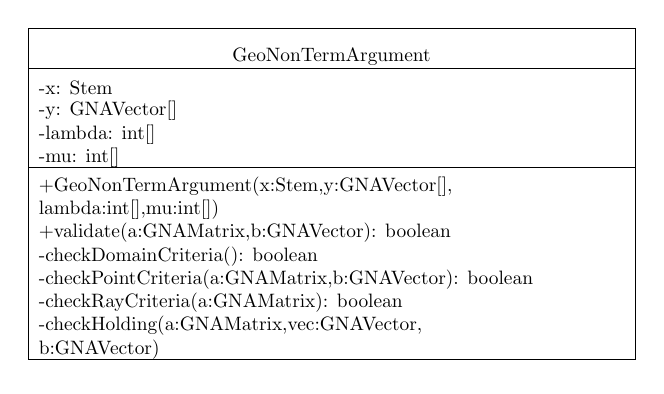
\begin{tikzpicture}[scale=0.7, every node/.style={scale=0.7}]
\pgftransformxscale{1.000000}
\pgftransformyscale{-1.000000}
\definecolor{dialinecolor}{rgb}{0.000000, 0.000000, 0.000000}
\pgfsetstrokecolor{dialinecolor}
\definecolor{dialinecolor}{rgb}{1.000000, 1.000000, 1.000000}
\pgfsetfillcolor{dialinecolor}
\pgfsetlinewidth{0.010000\du}
\pgfsetdash{}{0pt}
\definecolor{dialinecolor}{rgb}{1.000000, 1.000000, 1.000000}
\pgfsetfillcolor{dialinecolor}
\fill (8.645000\du,4.350000\du)--(8.645000\du,5.750000\du)--(29.550000\du,5.750000\du)--(29.550000\du,4.350000\du)--cycle;
\definecolor{dialinecolor}{rgb}{0.000000, 0.000000, 0.000000}
\pgfsetstrokecolor{dialinecolor}
\draw (8.645000\du,4.350000\du)--(8.645000\du,5.750000\du)--(29.550000\du,5.750000\du)--(29.550000\du,4.350000\du)--cycle;
% setfont left to latex
\definecolor{dialinecolor}{rgb}{0.000000, 0.000000, 0.000000}
\pgfsetstrokecolor{dialinecolor}
\node at (19.097500\du,5.350000\du){GeoNonTermArgument};
\definecolor{dialinecolor}{rgb}{1.000000, 1.000000, 1.000000}
\pgfsetfillcolor{dialinecolor}
\fill (8.645000\du,5.750000\du)--(8.645000\du,9.150000\du)--(29.550000\du,9.150000\du)--(29.550000\du,5.750000\du)--cycle;
\definecolor{dialinecolor}{rgb}{0.000000, 0.000000, 0.000000}
\pgfsetstrokecolor{dialinecolor}
\draw (8.645000\du,5.750000\du)--(8.645000\du,9.150000\du)--(29.550000\du,9.150000\du)--(29.550000\du,5.750000\du)--cycle;
% setfont left to latex
\definecolor{dialinecolor}{rgb}{0.000000, 0.000000, 0.000000}
\pgfsetstrokecolor{dialinecolor}
\node[anchor=west] at (8.795000\du,6.410000\du){-x: Stem};
% setfont left to latex
\definecolor{dialinecolor}{rgb}{0.000000, 0.000000, 0.000000}
\pgfsetstrokecolor{dialinecolor}
\node[anchor=west] at (8.795000\du,7.210000\du){-y: GNAVector\ensuremath{[}\ensuremath{]}};
% setfont left to latex
\definecolor{dialinecolor}{rgb}{0.000000, 0.000000, 0.000000}
\pgfsetstrokecolor{dialinecolor}
\node[anchor=west] at (8.795000\du,8.010000\du){-lambda: int\ensuremath{[}\ensuremath{]}};
% setfont left to latex
\definecolor{dialinecolor}{rgb}{0.000000, 0.000000, 0.000000}
\pgfsetstrokecolor{dialinecolor}
\node[anchor=west] at (8.795000\du,8.810000\du){-mu: int\ensuremath{[}\ensuremath{]}};
\definecolor{dialinecolor}{rgb}{1.000000, 1.000000, 1.000000}
\pgfsetfillcolor{dialinecolor}
\fill (8.645000\du,9.150000\du)--(8.645000\du,15.750000\du)--(29.550000\du,15.750000\du)--(29.550000\du,9.150000\du)--cycle;
\definecolor{dialinecolor}{rgb}{0.000000, 0.000000, 0.000000}
\pgfsetstrokecolor{dialinecolor}
\draw (8.645000\du,9.150000\du)--(8.645000\du,15.750000\du)--(29.550000\du,15.750000\du)--(29.550000\du,9.150000\du)--cycle;
% setfont left to latex
\definecolor{dialinecolor}{rgb}{0.000000, 0.000000, 0.000000}
\pgfsetstrokecolor{dialinecolor}
\node[anchor=west] at (8.795000\du,9.810000\du){+GeoNonTermArgument(x:Stem,y:GNAVector\ensuremath{[}\ensuremath{]},};
\definecolor{dialinecolor}{rgb}{0.000000, 0.000000, 0.000000}
\pgfsetstrokecolor{dialinecolor}
\node[anchor=west] at (8.795000\du,10.610000\du){                    lambda:int\ensuremath{[}\ensuremath{]},mu:int\ensuremath{[}\ensuremath{]})};
% setfont left to latex
\definecolor{dialinecolor}{rgb}{0.000000, 0.000000, 0.000000}
\pgfsetstrokecolor{dialinecolor}
\node[anchor=west] at (8.795000\du,11.410000\du){+validate(a:GNAMatrix,b:GNAVector): boolean};
% setfont left to latex
\definecolor{dialinecolor}{rgb}{0.000000, 0.000000, 0.000000}
\pgfsetstrokecolor{dialinecolor}
\node[anchor=west] at (8.795000\du,12.210000\du){-checkDomainCriteria(): boolean};
% setfont left to latex
\definecolor{dialinecolor}{rgb}{0.000000, 0.000000, 0.000000}
\pgfsetstrokecolor{dialinecolor}
\node[anchor=west] at (8.795000\du,13.010000\du){-checkPointCriteria(a:GNAMatrix,b:GNAVector): boolean};
% setfont left to latex
\definecolor{dialinecolor}{rgb}{0.000000, 0.000000, 0.000000}
\pgfsetstrokecolor{dialinecolor}
\node[anchor=west] at (8.795000\du,13.810000\du){-checkRayCriteria(a:GNAMatrix): boolean};
% setfont left to latex
\definecolor{dialinecolor}{rgb}{0.000000, 0.000000, 0.000000}
\pgfsetstrokecolor{dialinecolor}
\node[anchor=west] at (8.795000\du,14.610000\du){-checkHolding(a:GNAMatrix,vec:GNAVector,};
\definecolor{dialinecolor}{rgb}{0.000000, 0.000000, 0.000000}
\pgfsetstrokecolor{dialinecolor}
\node[anchor=west] at (8.795000\du,15.410000\du){              b:GNAVector)};
\end{tikzpicture}

	\caption{The \tool{Java}-class of a \gna given to \aprove as a witness of \nonterm}	
	\label{dia:gna-classdiagram}
\end{wrapfigure}
The implemented technique provides a model $m$ from the \solver and its assertions stated in \Cref{sec:derivation-smt}. From the model $m$ the technique filters the values and stores the in the \gna-class, which is given to \aprove as a witness. Such a \gna-object stores all variable declarations needed in order to revalidate itself to a given scenario. If one has an other technique of derivation it is possible to compute the matrices and set the values for a \gna-object and validate it, either proving it or mentioning, which criteria does not hold.\\ 
\\
\\
\\
From \Cref{chapter:geo-non-term} we get the following \iterationmatrix $A$ and \iterationconstants $b$: 
\begin{figure}[H]
	\centering
	$A=\begin{pmatrix}
		-1 		& -1 		&  0		& 0		 \\
		-1 		& 0 		&  0		& 0		 \\
		-3 		& 0 		&  0		& 0		 \\
		0 		& 2 		&  0		& 0		 \\
		3 		& 1 		&  -1		& 0		 \\
		0 		& 2 		&  0		& -1	 \\
		-3 		& -1 		&  1		& 0		 \\
		0 		& -2 		&  0		& 1	 	 \\
	\end{pmatrix}$	
	$b=\begin{pmatrix}
		-4 \\ -7 \\ -21 \\ -6 \\ 0 \\ 5 \\ 0 \\ -5
	\end{pmatrix}$
\end{figure}
The from the technique given witness is the \gna of size 2 with the following values:
\begin{figure}[H]
	\label{ex:gna}
	\centering
	\begin{tabular}{|c|c|c|c|c|c|}
		\hline
		\stem & $y_1$ & $y_2$ & $\lambda_1$ & $\lambda_2$ & $\mu_1$ \\ \hline
		$\begin{pmatrix} 10 \\ -3 \end{pmatrix}$ & $\begin{pmatrix} 9 \\ 0 \end{pmatrix}$ & $\begin{pmatrix} 8 \\ -8 \end{pmatrix}$ & 3 & 2 & 0 \\ \hline
	\end{tabular}
\end{figure}
From that we can start and validate every criteria stated in \Cref{def:gna}.

	\subsection[Verifying: domain-criteria]{(domain-criteria)	$x, y_1, \dots, y_k \in \mathbb{R}^n$, $\lambda_1, \dots \lambda_k, \mu_1, \dots \mu_{k-1} \ge 0$ }
		The validity of this criteria is given in \Cref{ex:gna} with $n=2$. This should not be surprising, since we defined the vectors to this dimension and the $\lambda$'s and $\mu$'s to be $\ge 0$ in \Cref{sec:derivation-smt}.
		
	\subsection[Verifying: init-criteria]{(init-criteria) x represents the \startterm (\stem)}
	Also the given \stem meets the conditions as already derived in \Cref{sec:stem-var}.
	
	\newsavebox{\pointcrit}% Box to store smallmatrix content
	\savebox{\pointcrit}{$A\begin{pmatrix} x \\ x + \sum_i y_i \end{pmatrix} \le b$}
	\subsection[Verifying: point-criteria]{(point-criteria) \usebox{\pointcrit} }
	
	Now we have to compute the sum of the $y_i$'s and observe if the inequation holds. So with the values given in \Cref{ex:gna} we receive:
	\begin{figure}[H]
		\centering
		$A\begin{pmatrix} x \\ x + \sum_i y_i \end{pmatrix} \le b \Leftrightarrow A\begin{pmatrix} 10 \\ -3 \\ 10 + (9+8) \\ -3 + (0+(-8))\end{pmatrix} \le b \Leftrightarrow A\begin{pmatrix} 10 \\ -3 \\ 27 \\ -11 \end{pmatrix} \le b \Leftrightarrow \begin{pmatrix} -7 \\ -10 \\ -30 \\ -6 \\ 0 \\ 5 \\ 0 \\ -5 \end{pmatrix} \le \begin{pmatrix}	-4 \\ -7 \\ -21 \\ -6 \\ 0 \\ 5 \\ 0 \\ -5 \end{pmatrix}$ 
	\end{figure}
	Not only one can see, that every row on its own satisfies the desired inequation, we can also observe the within \Cref{sec:point-criteria} stated equalities hold for the last $2n=2*2=4$ rows. The point-criteria obviously holds.

	\newsavebox{\raycrit}% Box to store smallmatrix content
	\savebox{\raycrit}{$A\begin{pmatrix} y_i \\ \lambda_i y_i + \mu_{i-1} y_{i-1} \end{pmatrix} \le 0$ for all $1 \le i \le k$}
	\subsection[Verifying: ray-criteria]{(ray-criteria) \usebox{\raycrit}}
	Because the \gna is of size $2$ we have only 2 ray-criteria sub-formulas that need to be tested
	\subsubsection{$r_1$: i=1}
	\begin{figure}[H]
		\centering
		$A\begin{pmatrix} y_1 \\ \lambda_1y_1 \end{pmatrix} \le 0 \Leftrightarrow A\begin{pmatrix} 9 \\ 0 \\ 3*9 \\ 3*0 \end{pmatrix} \le 0 \Leftrightarrow A\begin{pmatrix} 9 \\ 0 \\ 27 \\ 0 \end{pmatrix} \le 0 \Leftrightarrow \begin{pmatrix} -9 \\ -9 \\ -27 \\ 0 \\ 0 \\ 0 \\ 0 \\ 0 \end{pmatrix} \le \begin{pmatrix} 0 \\ 0 \\ 0 \\ 0 \\ 0 \\ 0 \\ 0 \\ 0 \end{pmatrix}$
	\end{figure}
	
	\subsubsection{$r_2$: i=2}
	\begin{figure}[H]
		\centering
		$A\begin{pmatrix} y_2 \\ \lambda_2y_2+\mu_1y_1 \end{pmatrix} \le 0 \Leftrightarrow A\begin{pmatrix} 8 \\ -8 \\ 2*8+0*9 \\ 2*(-8)+0*0 \end{pmatrix} \le 0 \Leftrightarrow A\begin{pmatrix} 8 \\ -8 \\ 16 \\ -16 \end{pmatrix} \le 0 \Leftrightarrow \begin{pmatrix} 0 \\ -8 \\ -24 \\ -16 \\ 0 \\ 0 \\ 0 \\ 0 \end{pmatrix} \le \begin{pmatrix} 0 \\ 0 \\ 0 \\ 0 \\ 0 \\ 0 \\ 0 \\ 0 \end{pmatrix}$
	\end{figure}

	Since all $r_i$ $1\le i \le 2$ are computed and checked that they hold also the ray-criteria holds.
	\\
	\\
	Observing that all criteria hold the whole \gna is suitable to \Cref{def:gna} and therefore is a witness of \nonterm regard the program stated in \Cref{fig:structure-example-java}.
	
